\documentclass{standalone}

\usepackage{tikz}
\begin{document}
  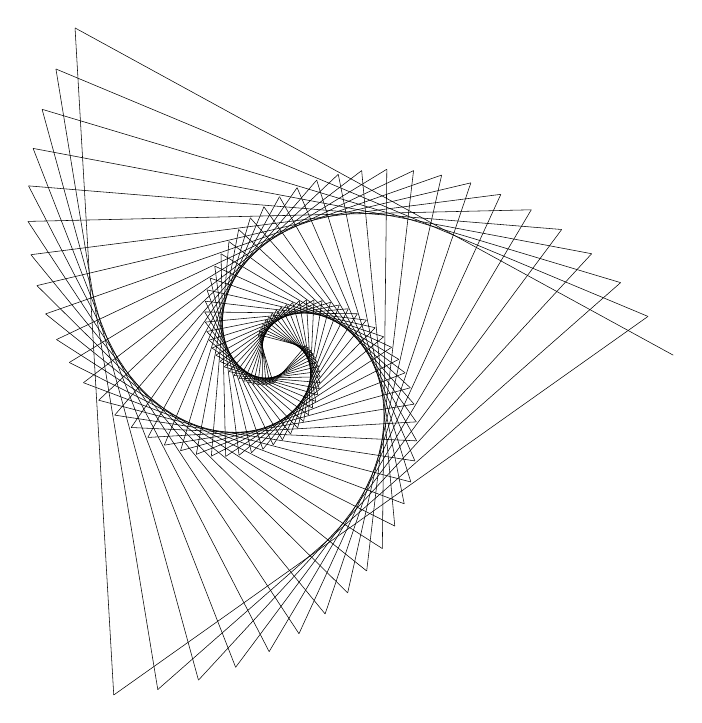
\begin{tikzpicture}
    \pgfmathsetmacro{\sc}{1}
    \pgfmathsetmacro{\an}{0}
    \foreach\i in {1,...,130} {
      \pgfmathsetmacro{\l}{5*\sc}
      \pgfmathsetmacro{\ax}{\l*cos(\an)}
      \pgfmathsetmacro{\ay}{\l*sin(\an)}

      \pgfmathsetmacro{\scx}{\sc*0.98}
      \pgfmathsetmacro{\anx}{\an+122}
      \pgfmathsetmacro{\l}{5*\scx}
      \pgfmathsetmacro{\bx}{\l*cos(\anx)}
      \pgfmathsetmacro{\by}{\l*sin(\anx)}

      \draw[very thin] (\ax,\ay) -- (\bx,\by);

      \global\let\sc=\scx
      \global\let\an=\anx
    }
  \end{tikzpicture}
\end{document}